\chapter{Objective specification and presentation of the research methodology}

Having laid the groundwork with essential concepts necessary for this thesis,
this chapter aims to outline the objectives of the practical segment as well as the research methodology employed to achieve them.
In the first part, the specific objectives are defined. 
Afterwards, in a second part the used reasearch framework \ac{DSR} and the two research methods Prototyping and the Simulation are explained.

\section{Objective specification}
The mentioned papers in 2.4.4 showed that the acceleration of statistical sampling in \ac{BM}s theoretically work. 
In order to answer the research question, this thesis wants to validate these proof of concepts in a first part and see if they are feasible on the complete \ac{ASIC} hardware accelerator like the \ac{mem-HNN}. 
The second practical part goes further and has the goal of implementing a simulator pipeline with the workload of a \ac{BM}
and meassure if it brings an actual acceleration. 
Currently, such a simulation model does not exist and would be able to extract data for further research and fundamental insights.  
Key metrics identified in the literature that demonstrate the performance of accelerators include throughput (samples/second) and energy consumption (energy/operation).\footnote{cf.\cite{caiPowerefficientCombinatorialOptimization2020}, p. 409-418; cf.\cite{ortega-zamoranoFPGAHardwareAcceleration2016}, p. 16-17; cf.\cite{aaditAcceleratingAdaptiveParallel2023}, p. 2; cf.\cite{bellettiJanusFPGABasedSystem2009}, p. 55}
Therefore, this is the goal of the data acquisition in the second practical part.
The practical part is therefore simulating a current \ac{ASIC} with not only the memristor crossbar array but also all the other requried hardware components.
Furthermore, the thesis focuses on an actual training of a \ac{RBM} and also the interference of it to answer the research question.
Expanding upon the foundational work, this research explores the implementation of the N/2 synchronous update mechanism.
This sampling method emphasizes a expactation of higher sampling speeds and efficiency.

At the beginning, the \ac{IT}-artifact to be implemented is modeled and all components, transitions and processes of the overall solution are identified.
Upon this ideal overall solution a prototyp is developed that impelments a subset of the real hardware functionalities.
As a result of the implementation a complete performance evaluation, including a comprehensive energy model and a latency model should be established.
The following simulation aims to measure the metrics: required processing time (samples/sec) for data and the energy usage (energy/operation).
The results should be compared to other sampling methods, such as Gibbs and Metropolis sampling.
Lastly, this thesis performs hyperparameter tuning in oder to gather new data on how these machines should be configured for optimal performance.
Since, there is no data for hyperparameter tuning of such a concept in the literature yet this establishes foundational work on how to make use of artificial intelligence within such an accelerator.
Through this process, the research seeks to determine the feasibility of a proper training with this setup, focusing on its practicality and efficiency.
By benchmarking these aspects against traditional sampling methods, the thesis aims to underscore the potential of the \ac{mem-HNN} 
in practical training of \ac{RBM}s.

Hence, \ac{DSR} is used as a research framework to iteratively create the \ac{IT}-artifact. 
In addition to that, within the single iterations prototyping is used for the actual implementation of the \ac{RBM} on the simulated \ac{mem-HNN} with individual goals.
The last iteration uses a simulation as research method because there the behaviour and performance of the system is meassured and the underlying model already finisehd with the last prototyping iteration. 
Since, the practical functionality can't be ensured the \ac{DSR} process combined with prototyping and if successful a simulation 
brings flexibility and a problem-oriented structure which are emphasized for this new method. 

\section{Design Science Research}

In terms of information systems \ac{DSR} is a core research method within the field of business informatics that ``creates and evaluates \ac{IT}-artifacts intended to solve identified organizational problems''.\footcite[77]{hevnerDesignScienceInformation2004a}
Henver et al. established a DSR framework that has the goal of creating an \ac{IT}-artifact which has the purpose of addressing and solving the important organizational problem.\footcite[82]{hevnerDesignScienceInformation2004a}
This systematic \ac{DSR} process lays a solid groundwork for conducting the research with rigor, offering a degree of confidence that the endeavor will yield meaningful outcomes.\footcite[cf.][368]{baskervilleDesignScienceResearch2018}
Artifacts in \ac{DSR} can be constructs, models, methods or instantiations.\footcite[77]{hevnerDesignScienceInformation2004a}
In addition to that, Gregor and Hevner (2013) categorize the underlying \ac{IT}-artifact based on their abstraction level and maturities.
Hence, level 1 represents a specific, limited and less mature implementation of an artifact, level 2 are operational principles or architecture like constructs, methods or models, while level 3 represents a well-developed midrange design theory.\footcite[cf.][342]{gregorPositioningPresentingDesign2013}
The development of the artifact is performed incrementally with specific goals for each iteration, which is beneficial for \ac{IT}-artifacts that can be adjusted after every iteration.\footcite[cf.][343]{gregorPositioningPresentingDesign2013}

Henver et al. also introduced 7 guidelines that still today serve as framework for different \ac{DSR} approaches.
Arguably, the most important two guidelines are, that the research must create a viable artifact that in a next step is able to solve the organizational problem. 
Another important guideline is that the artifact needs to be rigorously evaluated in utility, quality and efficiency.\footcite[83]{hevnerDesignScienceInformation2004a}
Thereupon Peffer et al. introduced a well-known \ac{DSR} Process Model, which has 6 different phases: Identify problem \& Motivate, Define Objectives of a solution, 
Design \& Development, Demonstration, Evaluation and Communication.\footcite[cf.][54]{peffersDesignScienceResearch2007a}
Another interesting approach by Österle et. al is called design-oriented business informatics. 
This \ac{DSR} method is used in this thesis for following reasons.
His approach compresses the phases of Peffer et al. into a more compact model and also gives a more detailed explanation of each phase while still complying with the guidelines established by Henver et al..\footcite[cf.][1-6]{oesterleMemorandumZurGestaltungsorientierten2010}
On top of this promising framework they created a \ac{DSR} model called consortial research.
It addresses problems for collaborative research in terms of access to practical knowledge, rapid change and practical orientation and a lack of support for knowledge transfer.\footcite[cf.][273-274]{oesterleKonsortialforschung2010}
Österle et al. aim to bridge the gap between the knowledge base of both science and practice, with a focus on evaluating and ensuring the reproducibility of research outcomes.\footcite[cf.][5]{oesterleMemorandumZurGestaltungsorientierten2010}
However, the individual phases of the research framework can also be implemented on their own and the best features 
of the research framework and especially the contents of the phases should be combined with its older framework of design-oriented business informatics.
As a result following model showed in figure \ref{DSR_Modell} is used:
\begin{figure}[H]
    \centering
    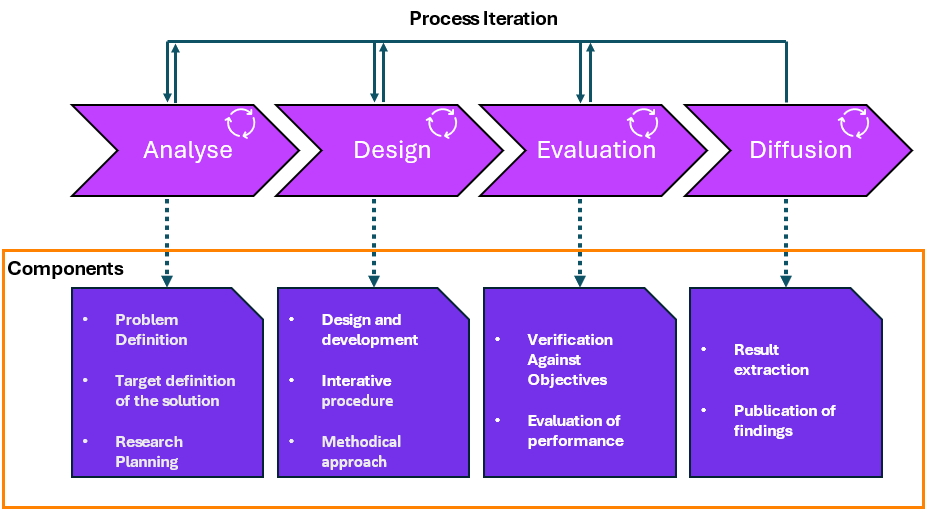
\includegraphics[width=0.9\linewidth]{graphics/DSR_Modell.png}
    \caption{\ac{DSR} model by Österle et. al\protect\footnotemark}
    \label{DSR_Modell}
\end{figure}
\footnotetext{inspired from \cite[cf.][278]{oesterleKonsortialforschung2010}}
This model uses an iterative process for the phases that allow backwards steps to redo an already completed phase if requriements were not satisfied to an appropriate level.
The four phases ideally contain the following contents:

\textbf{Analysis:} This phase identifies and describes the motivation in practice and formulates the desired research objectives.
In addition to that, a vague research plan is introduced which can hold goals of the project but also underlying constraints. 
Components of the research plan could be external stakeholders, funding, a timetable and of course a concept of the solution.
If possible also a research method should be selected.\footcite[cf.][4]{oesterleMemorandumZurGestaltungsorientierten2010}

\textbf{Design:} The \ac{IT}-artifact is designed and developed with regard to the selected research methology. 
Specific processes must be justified and comprehensible with consideration to the outcomes of the analysis phase.
The Design process can take multiple iterations on its own with the chance of making adjustments until the requirements.
The outcomes is a functional \ac{IT}-artifact that fulfills the set goals.\footcite[cf.][279]{oesterleKonsortialforschung2010}

\textbf{Evaluation:} Here the estasblished \ac{IT}-artifact needs to be validated against the earlier specified goals. 
Furthermore, it can be validated against the chosen research method. 
This means they must be applicable and they must provide the expected benefit.
If the artifact can not be testet with for example, an pilot application, it is poosible to persue expert interviews to validate the outcome.\footcite[cf.][279]{oesterleKonsortialforschung2010}

\textbf{Diffusion:} In this phase the results are generally made available to the public.
Therefore, the results need to be prepared for publication for individual communities.
Methods for publication could be teaching at universities and colleges and through their publication in books and specialist journals.
Diffusion in practice also includes the implementation in companies and public administration which the solution was initially developed for.\footcite[cf.][5]{oesterleMemorandumZurGestaltungsorientierten2010}

\section{Prototyping}

Given that the aim of the implementation is to create a new \ac{IT}-artifact with a focus on rapid development, prototyping has been selected as the methodology.
Generally, prototyping is a fundamental practice in designing tools, applications or user interfaces and defining requirements within the framework of agile software development.
It belongs to the agile requirements engineering practice and allows to gather feedback on requirements in a light-weight fashion.\footcite[cf.][1]{bjarnasonModelSoftwarePrototyping2021a}
Prototypes are created to assist in the analysis and design of proposed systems.
A prototype can be defined as ``a simplified model of a proposed system, that is built for a specific purpose'', which can apply to various kind of systems like software, hardware or even people.\footcite[][470]{luqiRapidSoftwarePrototyping1992}
It can be seen as an early increment, model, or release that implements some features of the desired product or model and therefore represents it. 

At the core of prototyping it comes down to the exploration of the solution space through experimenting with ideas,
collecting feedback and
communicating product requirements in an iteratively detailing process.
Hence, prototyping can deliver new requirements that are elicited through exploration and can later be validated 
by testing technical feasibility or business viability.\footcite[cf.][8]{bjarnasonModelSoftwarePrototyping2021a}
A few benefits of prototyping are early construction with low development costs and no large upfront investments of either time or money.
In addition to that, it can promote innovation due to early results that can be communicated and if viable researched further.\footcite[cf.][25]{nelsonSoftwarePrototyping2016}
The reason to chose prototyping can have various reasons. 
This thesis uses this method for the design phase within \ac{DSR} due to the just named benefits and the possibility of fast results and testing feasibility of the model.

In specific G. Arthur Mihram's prototyping model is chosen because it suits well to the \ac{DSR} framework and has overlaps with it. 
There are five steps to Mihram's prototyping process.
The first step, setting the ``modelling goals'' is already completed with the analysis phase of the \ac{DSR} analysis phase.\footcite[cf.][71]{mihramSimulationMethodology1976}
Within each iteration in the design phase a subselection of the goals are chosen to be prototyped. 
Furthermore, the previous established prototype is used as basis for the following iteration phase allowing to implement more and more features.
In a second step ``systemic analysis'', the prototype can be categorized to set the prototypes behavioural mechanisms.\footcite[cf.][71-72]{mihramSimulationMethodology1976}
As a guideline to categorize this behaviour the thesis uses the House of Prototyping Guidelines by Ahmed and Demirel.
These guidelines shown in \ref{attachement:prototyping_dimensions} introduce four different dimensions used to categorize prototypes:
Type of Prototype(1), Fidelity Level(2), Complexity(3), Scale(4) and Number of Iterations(5).\footcite[cf.][6-7]{ahmedPrototypingFrameworkHumanCentered2021}

The third step ``model synthesis'' requires a description and a chronological sequences of the prcoesses.\footcite[cf.][71-72]{mihramSimulationMethodology1976}
Furthermore, this is the phase of exploration and ends when the complete set of entities and the environment have been developed in a computer-directed language and the data is provided in machine-readable formats.\footcite[cf.][75-76]{mihramSimulationMethodology1976}

The last steps of Mihram's model: ``model confirmation'' and ``scientific interferenced'' are not considered since they overlap with the \ac{DSR} phases evaluation and diffusion. 
Simply this prevents a duplication of work.
Therefore, the categorization of the prototype and afterwards the ``model synthesis'' is executed per iteration in the prototyping model used in this thesis. 

\section{Simulation}

Simulation has been chosen as the methodology for the evaluation phase of the \ac{DSR} framework to collect data, due to the unavailability
of accelerators and the fact that the current chip design can be modeled more quickly and still accurate in software when done properly.
A simulation model can be defined as computerized representation of a given model capturing its dynamic behaviour.
The primary motivations for establishing a simulation model or using any other modeling method like prototyping is that it is
an cheap and fast way to gain important insights without being exposed to following constraints: costs, risks or logistics of manipulating the real system.\footcite[cf.][92]{kellnerSoftwareProcessSimulation1999}
Furthermore, the gathered data helps with decision making for strategical and operational levels.\footcite[cf.][93]{kellnerSoftwareProcessSimulation1999}
For example, with results of a simulation it can be decided if the new hardware works like expected and can be set up for production.
This are the reasons why the simulation methodology is chosen for the evaluation phase of the prototype. 

Computer simulation involves adjusting a computer-based model to better analyze how a system behaves and to evaluate approaches for their operation, either for descriptive or predictive purposes.\footcite[cf.][13-14]{abarAgentBasedModelling2017}
In the case of th \ac{mem-HNN}, there is the need for the evaluation of software performance in combination with the hardware to gather proper data.
The reason for this is that with only using a functional software simulation without considering the hardware specifications it results in a decreased price and time but with a significant precision loss.\footcite[cf.][470-471]{sarhadiStateArtHardware2015}
However, precision and efficiency are a key part towards beeing able to answer the research question.

A general simulation model by Kellner/Madachy/Raffo published a model that can be seen as overview of the work in the simulation field.
It consists out of the following entities: (0) model purpose, (1) model scope, (2) result variables, (3) process abstraction and (4) input parameters.  

\begin{figure}[H]
    \centering
    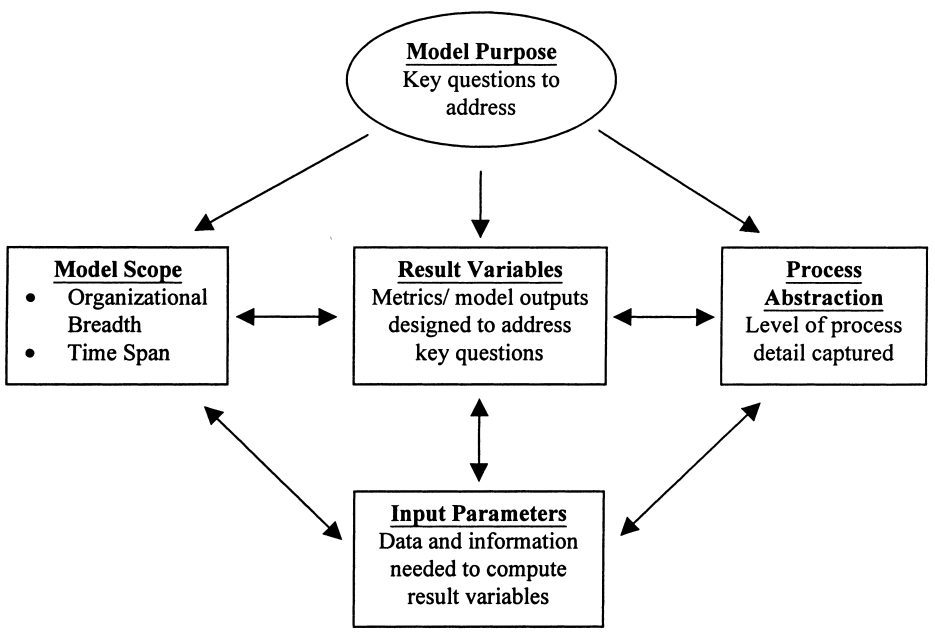
\includegraphics[width=0.7\linewidth]{graphics/Simulation_Modell.png}
    \caption{general simulation model\protect\footnotemark}
    \label{simulation_Modell}
\end{figure}
\footnotetext{\cite[][95]{kellnerSoftwareProcessSimulation1999}}

The general \textbf{model purpose} is based on the specific research question that needs to be answered.
It is crucial to thoroughly understand the effects based on this key question to ensure the correct selection of the \textbf{model scope}.\footcite[cf.][95]{kellnerSoftwareProcessSimulation1999}
This can be an iterative process which includes the selection of a scope, for example a development project, long-term product evolution etc. and within 
this scope an estimated timespan (short(less than 12 months), medium (12-24 months), long (more than 24months)) meeds to be selected. 
In addition to that, the organizational simulation breadth is set (less than one project team, one project team, multile project teams).\footcite[cf.][96]{kellnerSoftwareProcessSimulation1999}

The \textbf{result variables} are information elements that are the central key entity of the simulation model. 
They change based on the main question being asked, representing the crucial signs of a successful simulation.
Typical metrics for software simulation could be: effort/cost, throughput/productivity, queue lengths in the backlog,
energy efficiency, return on investment
Furthermore, with one simulation mutiple result variables can be gathered simultanously.\footcite[cf.][96-97]{kellnerSoftwareProcessSimulation1999}

\textbf{Process abstraction} includes inner structure of simulation model.
Therefroe, all the processes, vital ressources, dependencies and iteration looops need to be considered to achieve the desired result variables and to answer the key quesions.\footcite[cf.][97]{kellnerSoftwareProcessSimulation1999}
Lastly the \textbf{input parameters} consider all the parameters that are needed to produce vaulable outcomes. 
This can range up to hundreds of data parameters achieve the desired results. 
In theory, these parameters can also be extendetd to human ressources like software engineers that are needed for their skills in programming knowledge.\footcite[cf.][97-98]{kellnerSoftwareProcessSimulation1999}

This general usable simulation model should is not only part of the \ac{DSR} evaluation phase but also part of the \ac{ASIC} design process. 
Therefore, the model is modified to match the needs for a performance simlation of the \ac{mem-HNN}.
The simulation model is part of the architecture and high level design of the \ac{ASIC} design process.
It involves selecting key components like processors, memory blocks, and communication interfaces and carrying out a functional verification through a suitable simulation.\footnote{cf.\cite{raoUltimateGuideASIC}, p. 1; cf.\cite{ASICDesignFlow}, p. 1}
The modification to the model is expressed through the actual energy model of the \ac{mem-HNN}, which is added to the simulation model, that can compute energy usage per clock cycle. 
Hence, depending on a specific input it can calculate how much energy was required to do computations that are the output and used for the next cycle. 
